\documentclass[a4paper]{article}
\usepackage[utf8]{inputenc}
\usepackage{geometry}
\usepackage{amsmath}
\pdfpagewidth
\paperwidth
\pdfpageheight
\paperheight
\usepackage{booktabs}
\usepackage{graphicx}
\usepackage{subfig}
\usepackage{verbatim}
\newcommand*{\unit}[1]{\ensuremath{\mathrm{\,#1}}}
\usepackage{amsthm}
\usepackage{epsfig}
\usepackage{fancyhdr} 
\usepackage{amsmath,amssymb}
\usepackage{amscd} 
\usepackage[T1]{fontenc} 
\usepackage[utf8]{inputenc} 
\usepackage[usenames,dvipsnames]{xcolor}
\usepackage{graphicx,color,listings}
\usepackage{hologo}
\frenchspacing 
\usepackage{float}
\usepackage{geometry}
\usepackage{rotating}
\usepackage{caption}
\captionsetup{labelformat=empty, textfont=sl}
\usepackage{placeins}
\usepackage{hyperref}
\usepackage{listings}
\frenchspacing
\title{Esperienza Laboratorio di Fisica Medica: Esercizio di stima della risoluzione energetica di rivelatori a scintillazione}
\author{Jake Harold Pensavalle, Lorenzo Marini, Simone Lossano}
\begin{document}
	\maketitle
	\newpage
	\tableofcontents
	\newpage
%%%%%%%%%%%%%%%%%%%%%%%%%%%%%%%%%%%%%%
\section{Abstract}
Lo scopo di questa esperienza è trovare una metodologia che permetta di stimare la risoluzione energetica di rivelatori a scintillazione, in modo da massimizzare l'accordo con il valore predetto dalla simulazione con cui si sono ottenuti gli spettri. Il metodo più semplice è il fit gaussiano ma non è il migliore. Si intende massimizzare l'accordo cercato tramite un modello gaussiano con code esponenziali, un modello a doppia gaussiana e una modellizzazione del fondo di scattering con la formula di \textit{Klein-Nishina}.
\section{Introduzione}
Avendo a disposizione spettri generati da simulazioni si intende trovare il modello che meglio fitti le distribuzioni degli spettri, necessario per calcolare le risoluzioni energetiche con la formula:
\begin{equation}
Resolution=\frac{FWHM}{\mu}
\end{equation}
Dove $\mu$ è il canale centrale della distribuzione. Per lo spettro di BGO1F18 si conosce dalla simulazione la risoluzione, pari al $19.6\%$. Applichiamo a tutti gli spettri il modello che massimizza tale accordo.
\section{Analisi Dati}
Si procede facendo un istogramma normalizzato degli spettri e dalle prime analisi con modelli semplici, come il modello gaussiano, si nota un mancato accordo con il valore atteso. Ciò è dovuto alla presenza di fondo nella misura, e al fatto che lo spettro non è del tutto gaussiano. Consultando la letteratura fornita\footnote{\label{note1}"Introductory to Nuclear Physics", Kenneth S. Krane.} si evince che il fondo si può descrivere tramite un modello lineare, mentre lo spettro ha un andamento nelle code meglio descritto da un'esponenziale, dovuto alla presenza di componenti che decadono esponenzialmente. Consultando inoltre l'articolo fornito\footnote{\label{note2}"Positron Emission Tomography: Its 65 years"
A. Del Guerra, N. Belcari, M. Bisogni} risulta utile modellizzare il fondo di scattering compton tramite la formula di \textit{Klein-Nishina}.
Si decide dunque di procedere nell'utilizzo prima di un'esponenziale sommata alla gaussiana, o doppia gaussiana in base alla presenza di un picco aggiuntivo, in aggiunta al fondo descritto con un andamento lineare funzione con il canale ADC, in secondo luogo si studia l'aggiunta della funzione di Klein-Nishina al posto dell'esponenziale.
\subsection{La formula di Klein-Nishina}
Per modellizzare il fondo di scattering compton si utilizza la formula di Klein-Nishina a seguire:
\begin{equation}
\frac{d\sigma_{(\theta)}}{d\Omega}=r_{e}^{2}\frac{1+cos^{2}\theta}{2}\frac{1}{1+E_{\gamma}^{2}\left(1-cos\theta\right)^{2}}\left(1+\frac{E_{\gamma}\left(1-cos\theta\right)^{2}}{\left(1+cos^{2}\theta\right)\left(1+E_{\gamma}\left(1-cos\theta\right)}}\right)\right)
\end{equation}
dove $r_{e}$ è il raggio classico dell'elettrone, $E_{\gamma}$ è l'energia del raggio $\gamma$ incidente e $\theta$ è l'angolo di scattering.
Ricordando che l'energia residua $E^{'}_{\gamma}$ è data da:
\begin{equation}
E^{'}_{\gamma}=\frac{E_{\gamma}}{1+\left(\frac{E_{\gamma}}{m_{e}c^{2}}\right)\left(1-cos\theta\right)}
\end{equation}si può invertire questa relazione per ricavare $\cos\theta_{\left(E^{'}_{\gamma}\right)}$ e dunque fittare $\frac{d\sigma_{(E^{'}_{\gamma})}}{d\Omega}$ in funzione della ADC, che è legata a $E^{'}_{\gamma}$.
\subsection{Analisi con Python}
L'analisi è stata fatta con \textbf{Python} usando principalmente la libreria \textbf{lmfit}. Questa libreria ha un buon numero di funzioni implementate, di cui si distinguono le funzioni per la gaussiana \textbf{GaussianModel}, l'esponenziale \textbf{ExponentialModel} e il modello lineare \textbf{LinearModel}. Per l'analisi con la Klein-Nishina si definisce la funzione in funzione della ADC. Per facilitare la stima dei parametri iniziali e l'algoritmo di fit, si isolano i picchi per ogni istogramma. Di seguito si riporta il codice utilizzato. 
\begin{lstlisting}[language=Python]
import numpy as np
from lmfit.models import GaussianModel,ExponentialModel,LinearModel
from lmfit import Model
import os
import matplotlib.pyplot as plt

import glob
bins=200

#iniziamo il tutto caricando i dati
filenames=glob.glob('data*.txt')

###Ora definiamo la funzione di klein nishina

m_electron_c2=511 #in Kev
energy=511 #in Kev
r_e=8e-30 #raggio classico elettrone in m^2

def ferg(x):
    return m_electron_c2/energy+1-m_electron_c2/x
def Utility_1(x):
    return (1+ferg(x)**2)/2
def Utility_2(x):
    return 1/(1+(energy**2)*(1-ferg(x))**2)
def Utility_3(x):
    return (energy*(1-ferg(x))**2)/((1+ferg(x)**2)*(1+energy*(1-ferg(x))))

def kleinnishina(x):
    return r_e*Utility_1(x)*Utility_2(x)*(1+Utility_3(x))



for i in range(len(filenames)):
    f=filenames[i]
    pathsavefigure=('/Users/JakeHarold/Desktop/workplace/Gruppo-3-Lab-Fisica-Medica/BGORESOLUTION/latex/histklein%s.png'%f.replace('.txt',''))

    print(f)

    data=np.loadtxt(f,unpack=True)
#qui definisco gli estremi dei fotopicchi
[OMESSO]

#Inizializziamo l'istogramma

    plt.figure('%s'%f.replace('.txt',''))
    bin_heights, bin_borders, _=plt.hist(data,bins,facecolor='g',ec='black',alpha=0.5,label='histogram data',density=True)
    bin_centers = bin_borders[:-1] + np.diff(bin_borders) / 2
#qui creo il vettore per il fit sul fotopicco eliminando la parte che non interessa
    newcenters=[]
    newheights=[]
    for j in range(len(bin_heights)):
        if bin_centers[j]<b and bin_centers[j]>a:
            newcenters.append(bin_centers[j])
            newheights.append(bin_heights[j])
        else:
            pass
    y=np.array(newheights)
    x=np.array(newcenters)

#in base allo spettro, identificato da un indice che va da 0 a 10, fitto una gaussiana o una doppia gaussiana
    if i!=3 and i!=5:

        text='Gaussian Model w/ linear background & Expn. Decay'
        peak=GaussianModel()

    elif i==3 or i==5:
        text='Double Gaussian Model w/ linear background & Expn. Decay'
        peak1=GaussianModel(prefix='peak1')
        peak2=GaussianModel(prefix='peak2')
        peak=peak1+peak2

    noise=LinearModel()
#indovina i parametri iniziali
##Code Esponenziali
    tails=ExponentialModel(prefix='exp')
    mod=peak + noise + tails
    if i!=3 and i!=5:
        parspeak=peak.guess(y,x=x)

    elif i==3 or i==5 :

        parspeak1=peak1.guess(y,x=x)
        parspeak2=peak2.guess(y,x=x)
        parspeak=parspeak1+parspeak2

    else:
        print('ERROR GUESS')
    parslinear=noise.guess(y,x=x)

    parstails=tails.guess(y,x=x)
    pars=parspeak+parslinear+parstails
    out = mod.fit(y, pars, x=x)

    ##klein-Nishina

    klein=Model(kleinnishina)
    mod2=peak + klein +noise
    parss=parspeak+parslinear
    out2=mod2.fit(y,parss,x=x)

#ora calcoliamo le risoluzioni
###GAUSSIANA SINGOLA
    if i!=3 and i!=5:
        ##Exponential decay resolution
        fwhm=out.params['fwhm'].value
        center=out.params['center'].value
        resolution=100*fwhm/center
        ##Klein resolution
        fwhmk=out2.params['fwhm'].value
        centerk=out2.params['center'].value
        resolutionk=100*fwhmk/centerk
###DOPPIA GAUSSIANA
    elif i==3 or i==5:
        ##
        fwhm1=out.params['peak1fwhm'].value
        fwhm2=out.params['peak2fwhm'].value
        center1=out.params['peak1center'].value
        center2=out.params['peak2center'].value
        resolution1=100*fwhm1/center1
        resolution2=100*fwhm2/center2

        fwhm1k=out2.params['peak1fwhm'].value
        fwhm2k=out2.params['peak2fwhm'].value
        center1k=out2.params['peak1center'].value
        center2k=out2.params['peak2center'].value
        resolution1k=100*fwhm1k/center1k
        resolution2k=100*fwhm2k/center2k

    else:
        print('error')
# salviamo i risultati del fit su un txt
    with open('fit_result%s.txt'%f.replace('.txt',''), 'w') as fh:
        fh.write(out.fit_report())

    with open('fit_resultKlein%s.txt'%f.replace('.txt',''), 'w') as fh:
        fh.write(out2.fit_report())
[OMESSO]
\end{lstlisting}
Il codice per generare i file txt per il fit e il codice per l'analisi dati sono reperibili nel \href{https://github.com/Jake145/Gruppo-3-Lab-Fisica-Medica/tree/master/BGORESOLUTION}{\textbf{repositorio su github.}}
\section{Risultati}
\subsection{Gaussiana con fondo lineare e code gaussiane}
Utilizzando questo modello si è ottenuto un risultato di controllo promettente per il BGO1F18, infatti si stima una risoluzione energetica del $20.66\%$ a confronto con il $19.6\%$ dato dalla simulazione, che ha permesso di proseguire con il fit degli altri spettri con lo stesso modello. Nel caso del LSO1Ba133 e LSO2Ba133 essendovi due picchi si è utilizzato un modello a doppia gaussiana con riportate le rispettive risoluzioni
\subsection{Gaussiana con Klein-Nishina e fondo lineare}
Tra i due modelli questo metodo ha portato un accordo migliore col valore predetto. Infatti per il BGO1F18 si ottiene una risoluzione del $19.56\%$. Data la raffinatezza del modello, infatti risulta essere un passo in avanti rispetto al modello esponenziale, si reputa più probabile che i valori ottenuti con questo modello abbiano un accordo migliore col valore reale. Per il momento si è omessa l'applicazione sui doppi picchi in quanto è necessario migliorare la convergenza.
\begin{figure}[H]
\centering
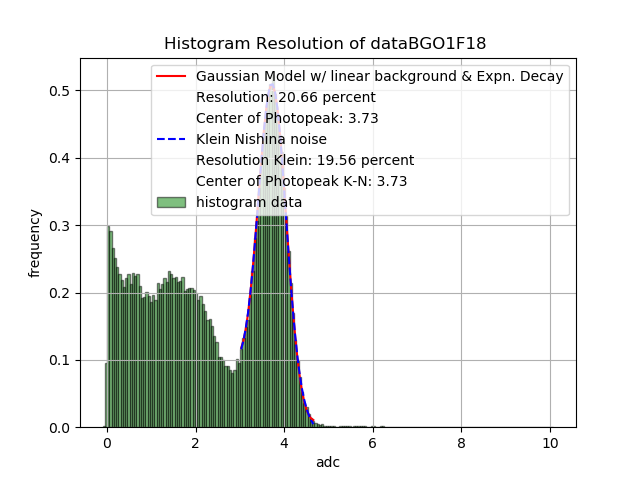
\includegraphics[width=0.75\textwidth]{histkleindataBGO1F18}
\caption{Figura 1: Risultati fit per il BGO1F18.}
\end{figure}
\begin{figure}[H]
\centering
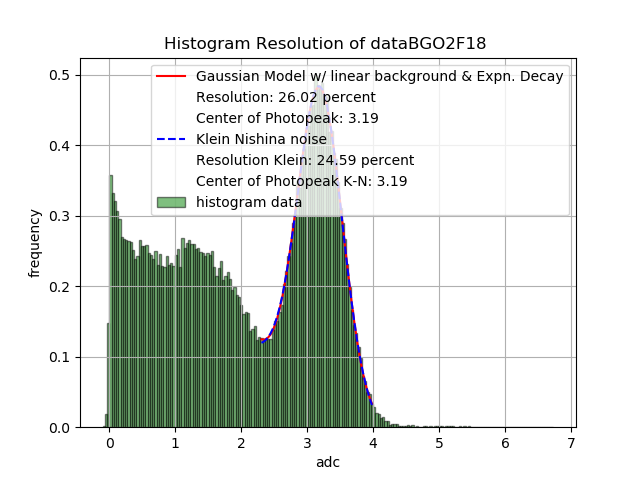
\includegraphics[width=0.75\textwidth]{histkleindataBGO2F18}
\caption{Figura 2: Risultati fit per il BGO2F18.}
\end{figure}
\begin{figure}[H]
\centering
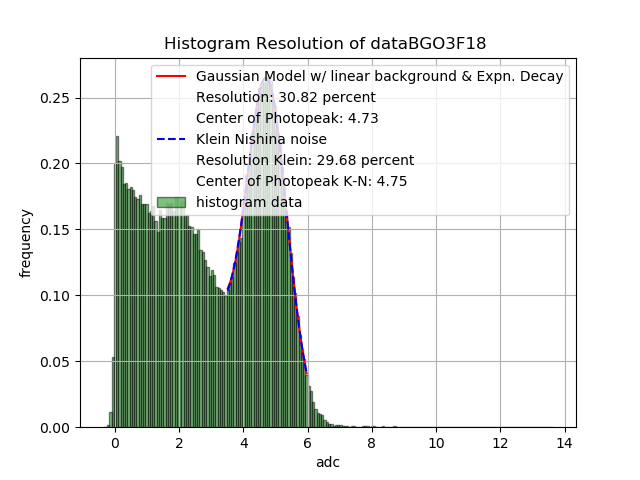
\includegraphics[width=0.75\textwidth]{histkleindataBGO3F18}
\caption{Figura 3: Risultati fit per il BGO3F18.}
\end{figure}
\begin{figure}[H]
\centering
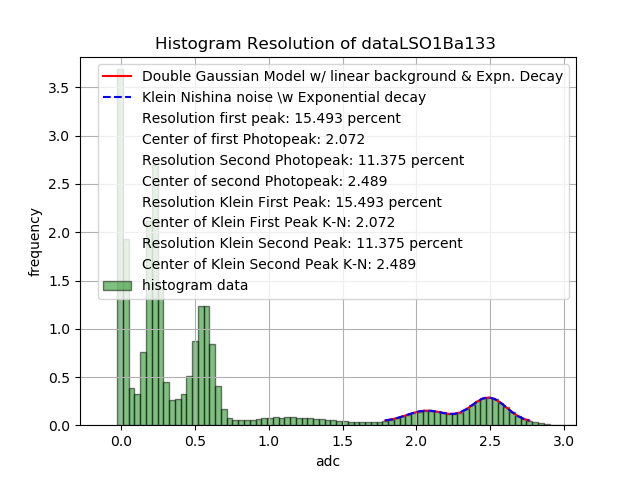
\includegraphics[width=0.75\textwidth]{histdataLSO1Ba133}
\caption{Figura 4: Risultati fit per il LSO1Ba133.}
\end{figure}

\begin{figure}[H]
\centering
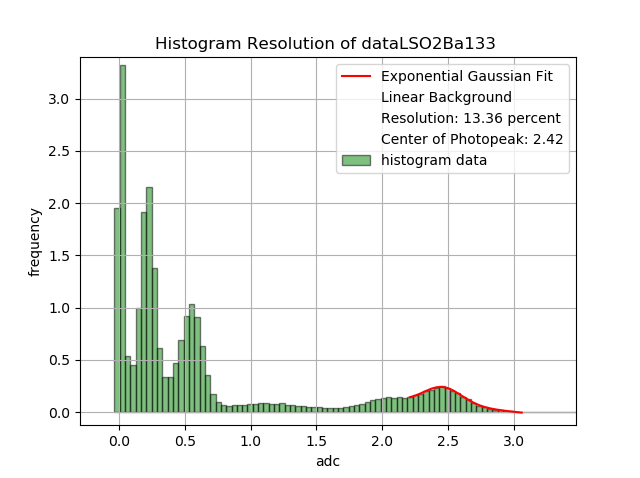
\includegraphics[width=0.75\textwidth]{histdataLSO2Ba133}
\caption{Figura 5: Risultato fit per il LSO2Ba133.}
\end{figure}
\begin{figure}[H]
\centering
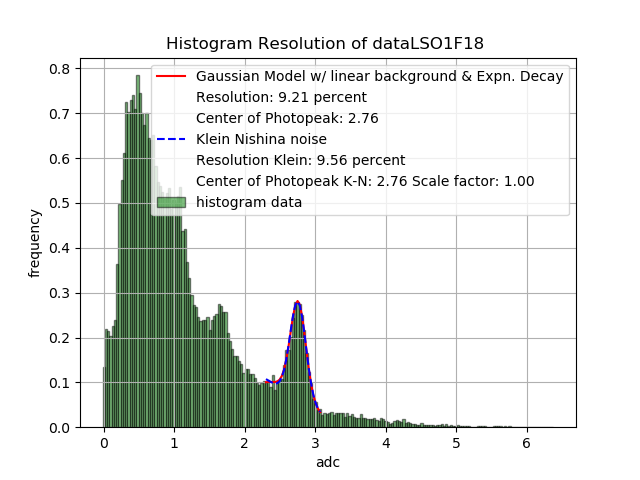
\includegraphics[width=0.75\textwidth]{histkleindataLSO1F18}
\caption{Figura 6: Risultati fit per il LSO1F18.}
\end{figure}
\begin{figure}[H]
\centering
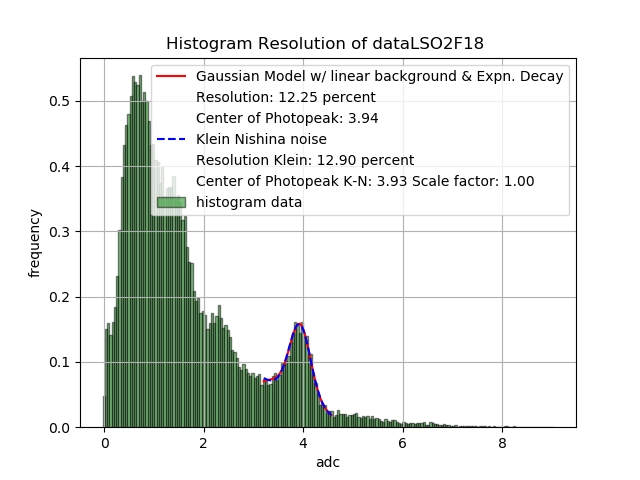
\includegraphics[width=0.75\textwidth]{histkleindataLSO2F18}
\caption{Figura 7: Risultato fit per il LSO2F18.}
\end{figure}
\begin{figure}[H]
\centering
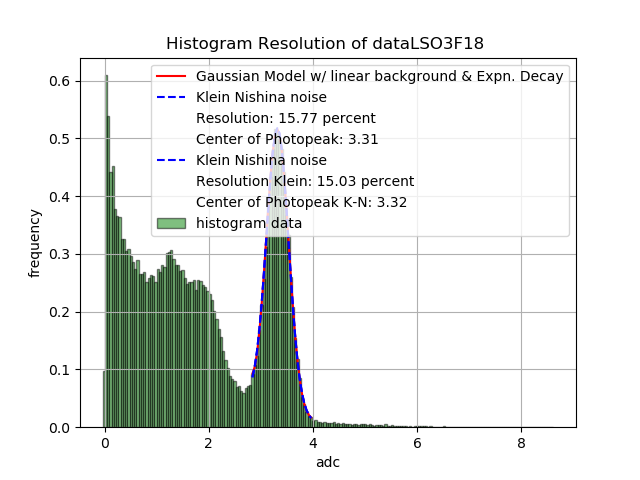
\includegraphics[width=0.75\textwidth]{histkleindataLSO3F18}
\caption{Figura 8: Risultato fit per il LSO3F18.}
\end{figure}
\begin{figure}[H]
\centering
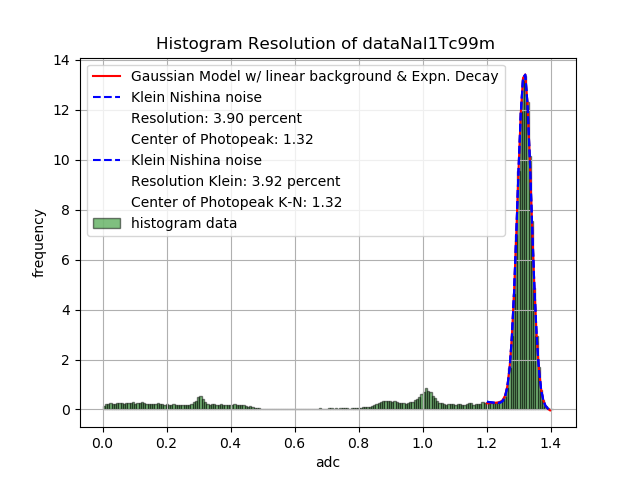
\includegraphics[width=0.75\textwidth]{histkleindataNaI1Tc99m}
\caption{Figura 9: Risultato fit per il NaI1Tc99m}
\end{figure}
\begin{figure}[H]
\centering
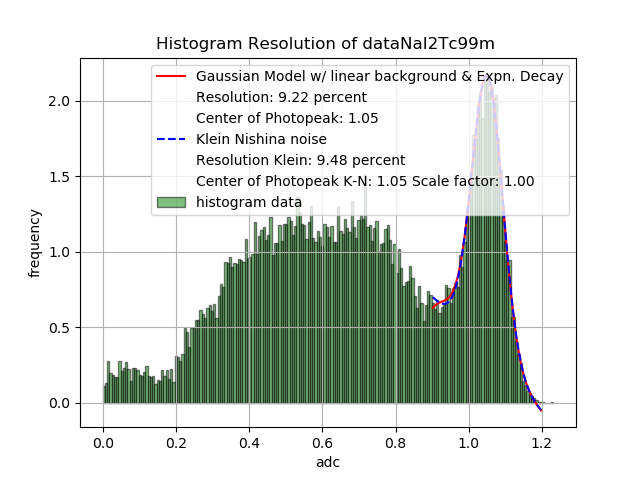
\includegraphics[width=0.75\textwidth]{histkleindataNaI2Tc99m}
\caption{Figura 10: Risultato fit per il NaI2Tc99m}
\end{figure}
\begin{figure}[H]
\centering
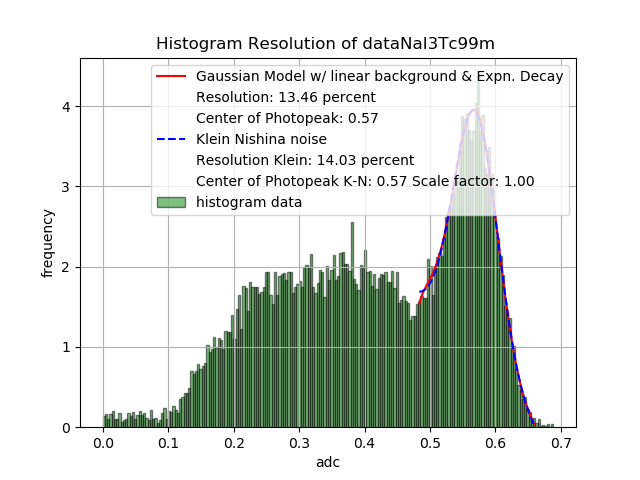
\includegraphics[width=0.75\textwidth]{histkleindataNaI3Tc99m}
\caption{Figura 11: Risultato fit per il NaI3Tc99m}
\end{figure}
\end{document}